\documentclass{beamer}

\mode<presentation> {
\usetheme{Boadilla}
\usecolortheme{default}
\usefonttheme[onlymath]{serif}
}
\usepackage{amsmath}
\usepackage{amssymb}
\usepackage{amsthm}
\usepackage{mathtools}
\usepackage{caption}
\usepackage{hyperref}
\usepackage{booktabs}
\usepackage{array} 
\usepackage{filecontents}
\usepackage{pgfplots, pgfplotstable}


\pgfplotsset{compat=1.16}
\usepackage[USenglish,british,american,australian,english]{babel}
\begin{filecontents}{\jobname.bib}
@article{smith2002tutorial,
  title={A tutorial on principal components analysis},
  author={Smith, Lindsay I},
  year={2002}
}

@book{anton2013elementary,
  title={Elementary linear algebra: applications version},
  author={Anton, Howard and Rorres, Chris},
  year={2013},
  publisher={John Wiley \& Sons}
}
\end{filecontents}
\usepackage[style=numeric,backend=biber,autocite=plain,sorting=none]{biblatex}
\addbibresource{\jobname.bib}
  
\usepackage{graphicx} % Allows including images

\usepackage{booktabs} % Allows the use of \toprule, 
\usepackage{listings}
\usepackage{minted}
\usepackage{tikz}
%\usepackage{etoolbox} % for \ifthen
\usepackage{listofitems} % for \readlist to create arrays
\usetikzlibrary{datavisualization, arrows.meta, shapes, shadows, arrows} % for arrow size
\usepackage[outline]{contour} % glow around text
\contourlength{1.4pt}

\tikzset{>=latex, >={Straight Barb[angle'=80, scale=1.1]}} % for LaTeX arrow head
\usepackage{xcolor}

\definecolor{green}{rgb}{0.0,0.50,0.0}

% Scientific libs


\def\nstyle{int(\lay<\Nnodlen?min(2,\lay):3)} % map layer number onto 1, 2, or 3
\DeclareMathOperator*{\argmax}{arg\,max}
\DeclareMathOperator*{\argmin}{arg\,min}
\setbeamertemplate{caption}[numbered]
\AtBeginBibliography{\small}

\tikzstyle{decision} = [diamond, draw, fill=white]
\tikzstyle{line} = [draw, -stealth, thick]
\tikzstyle{elli}=[draw, ellipse, fill=gray!20, minimum height=8mm, text width=5em, text centered]
\tikzstyle{block} = [draw, rectangle, fill=white, text width=8em, text centered, minimum height=15mm, node distance=10em]

%Includes "References" in the table of contents

\title[CodeSeoul] % (optional, only for long titles)
  {Dimensionality reduction techniques: \\Part 2}

\author[Machine Learning Afternoons] % (optional, for multiple authors)
  {Sanzhar Askaruly (San)}

\institute[] % (optional)
  { Ulsan National Institute of Science and Technology\newline
    Ph.D. Candidate in Biomedical Engineering}

\date[December 24]
{CodeSeoul MLA \\December 24, 2022}

% some change
\begin{document}
    %\maketitle
    \begin{frame}
    \titlepage % Print the title page as the first slide
    \end{frame}

    \begin{frame}
        \frametitle{Last time...}
        \begin{center}
            \includegraphics[width=1.0\textwidth]{/home/suzy/gitrepos/tuttelikz/machine-learning/221224-tsne/images/last_time.png}
        \end{center}
    \end{frame}

    \begin{frame}{Today}
      \tableofcontents
    \end{frame}

    
    \section{Problem with linear methods}
    \begin{frame}{Dimensionality reduction}
        \begin{center}
            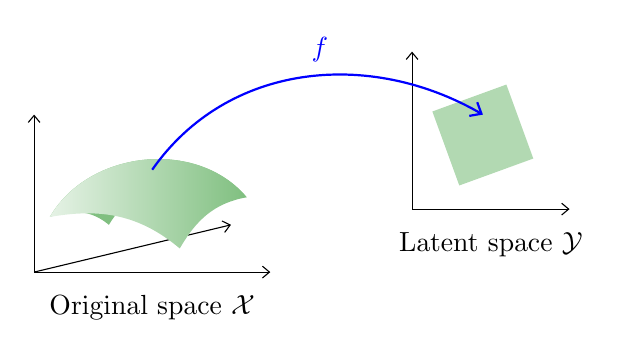
\begin{tikzpicture}

                \draw[->] (0, 0) -- ++(0, 2);
                \draw[->] (0, 0) -- ++(2.5, 0.6);
                \draw[->] (0, 0) -- ++(3, 0) node[midway, below, yshift=-0.5em]
                    {Original space ${\cal X}$};
                
                \draw[fill=green!50, draw=none, shift={(0.2, 0.7)},scale=0.5]
                  (0, 0) to[out=20, in=140] (1.5, -0.2) to [out=60, in=160]
                  (5, 0.5) to[out=130, in=60]
                  cycle;
                
                \shade[thin, left color=green!10, right color=green!50, draw=none,
                  shift={(0.2, 0.7)},scale=0.5]
                  (0, 0) to[out=10, in=140] (3.3, -0.8) to [out=60, in=190] (5, 0.5)
                    to[out=130, in=60] cycle;
                
                  \draw[->] (4.8, 0.8) -- ++(0, 2);
                  \draw[->] (4.8, 0.8) -- ++(2, 0) node[midway, below, yshift=-0.5em]
                      {Latent space ${\cal Y}$};
                
                  \draw[thin, fill=green!30, draw=none, shift={(5.4, 1.1)}, rotate=20]
                    (0, 0) -- (1, 0) -- (1, 1) -- (0, 1) -- cycle;
                
                  \draw[thick,->,blue]
                    (1.5, 1.3) to [out=55, in=150] node[midway, above, xshift=6pt, yshift=2pt]
                    {$f$} (5.7, 2);
                
                
                \end{tikzpicture}
        \end{center}
        \bigskip
        \begin{center}
            $$X=\{x_1, x_2, ..., x_n \in \mathbb{R}^{high}\} \rightarrow Y=\{y_1, y_2, ..., y_n \in \mathbb{R}^{low}\}$$
            $$\min_{Y}C(X,Y)$$
        \end{center}        
      \end{frame}
    
    \begin{frame}[fragile]
        \frametitle{Dimensionality reduction}
        Let's consider a \textbf{manifold}\footnote{a generalization of a curved surface; it is a topological space that is modeled closely on Euclidean space locally but may vary widely in global properties.} embedded nonlinearly in high-dim. space:\\~\\
        \begin{center}
            \includegraphics[width=0.9\textwidth]{/home/suzy/gitrepos/tuttelikz/machine-learning/221224-tsne/images/nonlinear_manifold_ex.png}
        \end{center}
        
    \end{frame}

    \begin{frame}[fragile]
        \frametitle{Dimensionality reduction}
        \begin{itemize}
            \item Linear projection may not be good enough..
        \end{itemize}
        \bigskip
        \begin{columns}
            \begin{column}{0.35\textwidth}
                \includegraphics[width=0.9\textwidth]{/home/suzy/gitrepos/tuttelikz/machine-learning/221224-tsne/images/swiss_roll.png}
            \end{column}
            \begin{column}{0.2\textwidth}
                \begin{center}
                    $\xrightarrow[\text{Linear projection}]{}$    
                \end{center}
                
                % \begin{tikzpicture}
                %     \coordinate (a) at (0,0);
                %     \coordinate (b) at (2,0);
                %     \draw[->, >=latex, blue!20!white, line width=15pt] (a) to node[black]{Linear projection} (b);
                % \end{tikzpicture}
            \end{column}
            \begin{column}{0.35\textwidth}
                \includegraphics[width=0.9\textwidth]{/home/suzy/gitrepos/tuttelikz/machine-learning/221224-tsne/images/linear_projection.png}
            \end{column}
            %\includegraphics[width=0.9\textwidth]{/home/suzy/gitrepos/tuttelikz/machine-learning/221224-tsne/images/nonlinear_manifold_ex.png}
        \end{columns}
        \bigskip
        \begin{itemize}
            \item Linear projection methods (\textit{eg.} PCA) \textcolor{red}{can't} capture intrinsic nonlinearities
        \end{itemize}
    \end{frame}

    \begin{frame}[fragile]
        \frametitle{Dimensionality reduction}
        \begin{itemize}
            \item Different criteria could be used for such projections
        \end{itemize}
        \bigskip
        \begin{columns}
            \begin{column}{0.35\textwidth}
                \includegraphics[width=0.9\textwidth]{/home/suzy/gitrepos/tuttelikz/machine-learning/221224-tsne/images/swiss_roll.png}
            \end{column}
            \begin{column}{0.2\textwidth}
                \begin{center}
                    $\xrightarrow[\text{Nonlinear projection}]{}$    
                \end{center}
                
                % \begin{tikzpicture}
                %     \coordinate (a) at (0,0);
                %     \coordinate (b) at (2,0);
                %     \draw[->, >=latex, blue!20!white, line width=15pt] (a) to node[black]{Linear projection} (b);
                % \end{tikzpicture}
            \end{column}
            \begin{column}{0.35\textwidth}
                \includegraphics[width=0.9\textwidth]{/home/suzy/gitrepos/tuttelikz/machine-learning/221224-tsne/images/nonlinear_projection.png}
            \end{column}
            %\includegraphics[width=0.9\textwidth]{/home/suzy/gitrepos/tuttelikz/machine-learning/221224-tsne/images/nonlinear_manifold_ex.png}
        \end{columns}
        \bigskip
        \begin{itemize}
            \item \textcolor{blue}{Preserve neighborhood information}
            \begin{itemize}
                \item Locally linear structures
                \item Pairwise distances
            \end{itemize}
        \end{itemize}
        
    \end{frame}

    \section{Non-linear methods (Manifold learning)}
    \subsection{SNE}
    

    \begin{frame}
        \frametitle{SNE: Idea}
        \textbf{How similar} is datapoint $x_j$ to datapoint $x_i$ in a high-dimesional space?\\~\\
        
        \begin{center}
            $$p_{j|i}=\frac{exp{(-||x^{(i)}-x^{(j)}||^2/2\sigma_i^2)}}{
                \sum_{k\not=i}^{} exp{(-||x^{(i)}-x^{(k)}||^2/2\sigma_i^2)}}$$
        \end{center}
        \bigskip
        SNE uses Euclidian distance to estimate the probability (according to Gaussian) of similarity between neighbor datapoints $x_i$ and $x_j$
    \end{frame}


    \begin{frame}
        \frametitle{SNE: Idea}
        \textbf{How similar} is datapoint $y_j$ to datapoint $y_i$ in a low-dimesional space?\\~\\
        
        \begin{center}
            $$q_{j|i}=\frac{exp{(-||y^{(i)}-y^{(j)}||^2/2\sigma_i^2)}}{
                \sum_{k\not=i}^{} exp{(-||y^{(i)}-y^{(k)}||^2/2\sigma_i^2)}}$$
        \end{center}
        \bigskip
        Similarly to HD, SNE uses Euclidian distance to estimate the probability of similarity between neighbor datapoints $y_i$ and $y_j$
    \end{frame}


    \begin{frame}{SNE: Example}
        \begin{center}
            \includegraphics[width=1.0\textwidth]{/home/suzy/gitrepos/tuttelikz/machine-learning/221224-tsne/images/illu1.png}
        \end{center}
    \end{frame}
    \begin{frame}{SNE: Example}
        \begin{center}
            \includegraphics[width=1.0\textwidth]{/home/suzy/gitrepos/tuttelikz/machine-learning/221224-tsne/images/illu2.png}
        \end{center}
    \end{frame}
    \begin{frame}{SNE: Example}
        \begin{center}
            \includegraphics[width=1.0\textwidth]{/home/suzy/gitrepos/tuttelikz/machine-learning/221224-tsne/images/illu3.png}
        \end{center}
    \end{frame}
    \begin{frame}{SNE: Example}
        \begin{center}
            \includegraphics[width=1.0\textwidth]{/home/suzy/gitrepos/tuttelikz/machine-learning/221224-tsne/images/illu4.png}
        \end{center}
    \end{frame}
    \begin{frame}{SNE: Example}
        \begin{center}
            \includegraphics[width=1.0\textwidth]{/home/suzy/gitrepos/tuttelikz/machine-learning/221224-tsne/images/illu5.png}
        \end{center}
    \end{frame}

    \begin{frame}
        \frametitle{SNE: Principle}
        \begin{itemize}
            \item KL divergence compares the distributions on the neighbors:
        \end{itemize}
        
        \begin{center}
            $$C=\sum_{i}^{} KL(P_i||Q_i) = \sum_{i}^{}\sum_{j}^{} p_{j|i}\log{\frac{p_{j|i}}{q_{j|i}}}$$
        \end{center}
        \bigskip
        \begin{itemize}
            \item Minimization problem $\min_{y}{C(X,Y)}$
            \item Assymetric
            \item Always positive
        \end{itemize}
    \end{frame}


    \begin{frame}
        \frametitle{SNE: Principle}
        \begin{itemize}
            \item KL divergence compares the distributions on the neighbors:
        \end{itemize}
        
        \begin{center}
            $$C=\sum_{i}^{} KL(P_i||Q_i) = \sum_{i}^{}\sum_{j}^{} p_{j|i}\log{\frac{p_{j|i}}{q_{j|i}}}$$
        \end{center}
        \bigskip
        Minimization of this cost function is performed using gradient descent:
        \begin{center}
            $$\frac{\delta{C}}{\delta{y_i}}=2\sum_{j}^{} (p_{j|i} - {q_{j|i}} + p_{i|j} - {q_{i|j}})(y_i-y_j)$$
        \end{center}

    \end{frame}

    \begin{frame}
        \frametitle{SNE: Principle}
        
        \begin{center}
            \includegraphics[width=1.0\textwidth]{/home/suzy/gitrepos/tuttelikz/machine-learning/221224-tsne/images/opt_momentum.png}
        \end{center}
        
        Mathematically, the gradient update with a momentum term is given by:

        \begin{center}
            $$Y^{(t)}=Y^{(t-1)} + \mu\frac{\delta{C}}{\delta{Y}} + \alpha(t) \left(Y^{(t-1)} - Y^{(t-2)} \right)$$
        \end{center}

    \end{frame}

    
    \subsection{t-SNE}

    \begin{frame}
        \frametitle{Crowding problem}
    \end{frame}

    \begin{frame}
        \frametitle{tSNE}
        \textbf{How similar} is datapoint $y_j$ to datapoint $y_i$ in a low-dimesional space?\\~\\
        
        \begin{center}
            $$q_{j|i}=\frac{(1+||y_i-y_j||^2)^{-1}}{\sum_{k\not=l}^{}(1+||y_i-y_j||^2)^{-1}}$$
        \end{center}
        \bigskip
        In low-dimension, the Gaussian distribution is replaced by student T-distribution
    \end{frame}
    \begin{frame}
        \frametitle{SNE: Principle}
        \begin{itemize}
            \item KL divergence compares the distributions on the neighbors:
        \end{itemize}
        
        \begin{center}
            $$C=\sum_{i}^{} KL(P||Q) = \sum_{i}^{}\sum_{j}^{} p_{ij}\log{\frac{p_{ij}}{q_{ji}}}$$
        \end{center}
        \bigskip
        Minimization of this cost function is performed using gradient descent:
        \begin{center}
            $$\frac{\delta{C}}{\delta{y_i}}=4\sum_{j}^{} (p_{ij} - {q_{ji}})(y_i-y_j)(1+||y_i-y_j||^2)^{-1}$$
        \end{center}

    \end{frame}

    
    \begin{frame}
        \frametitle{tSNE}
        \begin{columns}
            \begin{column}{0.5\textwidth}
                \includegraphics[width=1.0\textwidth]{/home/suzy/gitrepos/tuttelikz/machine-learning/221224-tsne/images/sne_gradient.png}        
            \end{column}

            \begin{column}{0.5\textwidth}
                \includegraphics[width=1.0\textwidth]{/home/suzy/gitrepos/tuttelikz/machine-learning/221224-tsne/images/tsne_gradient.png}        
            \end{column}
        \end{columns}
    \end{frame}

    \begin{frame}
        \frametitle{Algorithm}
        \includegraphics[width=1.0\textwidth]{/home/suzy/gitrepos/tuttelikz/machine-learning/221224-tsne/images/tsne_algo.png}
        
    \end{frame}

    \subsection{Isomap}
    \begin{frame}
        https://www.andrew.cmu.edu/user/georgech/95-865/        
    \end{frame}


    

    %mark=o,greenmark options={fill=red}

    \nocite{*}

    % \section{Summary} %
    % \subsection{Conclusion}
    % \begin{frame}{Conclusion}

    % \end{frame}


    \section{Further}
    \subsection{Lecture contents}
    \begin{frame}{}
      \begin{center}
      \begin{huge}Thank you for your attention!\end{huge}
      \end{center}
    \end{frame}
    %http://colah.github.io/posts/2014-10-Visualizing-MNIST/#fn2
    % https://scikit-learn.org/stable/auto_examples/manifold/plot_lle_digits.html
    % https://www.andrew.cmu.edu/user/georgech/95-865/
    % https://docs.google.com/presentation/d/1uOWkXVdEL_P9kO-kCmjkeLdVGR-oYb-3_mLlXp0Ezs8/edit#slide=id.p
    % https://fleuret.org/dlc/
    \subsection{References}
    % \begin{frame}{References}
    %   \printbibliography
    % \end{frame}

\end{document}
